\documentclass[12pt]{article}
\usepackage{fullpage}
\usepackage{graphicx, rotating, booktabs} 
\usepackage{times} 
\usepackage{fbb} 
\usepackage{natbib} 
\usepackage{indentfirst} 
\usepackage{setspace}
\usepackage{grffile} 
\usepackage{hyperref}
\usepackage{tikz-cd}
 \usetikzlibrary{cd}
\usepackage[export]{adjustbox}
\usepackage[most]{tcolorbox}
\usepackage{verbatimbox}
\usepackage{lscape}
\usepackage{afterpage}
\usepackage{amsmath}
\usepackage[labelfont={bf},textfont=it,labelsep=period]{caption}
 \usepackage{multirow} 
\setcitestyle{aysep{}}
\usepackage{dcolumn}

\hypersetup{
  colorlinks = true,
  urlcolor = blue,
  linkcolor = black,
  citecolor = black,
  pdfauthor = {Joshua Alley},
  pdfkeywords = {},
  pdftitle = {},
  pdfsubject = {},
  pdfpagemode = UseNone,
%  pdffitwindow = true
%  pdfcenterwindow = true
}



\singlespace
\title{\textbf{Using Bayesian Hierarchical Models to Estimate Heterogeneous Effects}}
\author{Joshua Alley \\
Assistant Professor \\
University College Dublin\thanks{Thanks to Carlisle Rainey for helpful comments.} \\
joshua.alley@ucd.ie
}

 
\date{\today}

\bibliographystyle{apsr}

\usepackage{sectsty}
\sectionfont{\Large}
\subsectionfont{\noindent\large\textit}
\subsubsectionfont{\normalsize}

\makeatletter
\renewcommand\tiny{\@setfontsize\tiny{9}{10}}
\makeatother


\begin{document}

\maketitle 

\begin{abstract} 
Heterogeneous effects are common in social science. 
In this note, I introduce a Bayesian hierarchical approach to estimating heterogeneous effects. 
The modeling strategy uses varying slopes and intercepts, along with predictors of the slopes, to capture heterogeneous effects by groups.  
Researchers can specify groups and sources of heterogeneity based on the quantities of interest, including heterogeneous treatments, treatment heterogeneity, and policy.  
This approach provides an intermediate tool between interactions or subgroup analyses and machine-learning approaches for discovering complex heterogeneity. 
It is more flexible than interactions and reduces the risk of underpowered subgroup comparisons.
At the same time, it is more theoretically driven and interpretable than some machine-learning approaches, as well as easier to implement in small datasets. 
Researchers can thus use hierarchical models alongside other approaches to understand heterogeneous effects for scholarship and policy.
\end{abstract} 


\newpage 
\doublespace 


\section{Introduction}


% one: het effects matter
Whether in observational and experimental studies, every independent variable social scientists examine impacts some units more or less than others. 
Aggregate relationships often mask heterogeneous effects.\footnote{For example, \citet{Abramsonetal2022} note that the average marginal component effect (AMCE) of conjoint experiments reflects the direction and intensity of respondent preferences, and gives more weight to intense preferences.} 
These averages are useful in some instances, but they often obscure interesting and important variation. 


As a result, understanding varying responses to a given stimulus is essential for policy and scholarship. 
Estimating heterogeneity allows scholars to better elucidate the process linking their independent variable and outcome.
Policymakers can target finite resources and focus interventions where they will have the most impact. 

% expand/sharpen this 

% two: introduce my solution 
This note introduces a hierarchical Bayesian approach to estimating heterogeneous effects. 
The technique estimates heterogeneous effects using varying slopes and intercepts, along with covariates that predict slopes. 
Modeling heterogeneous effects in this way is produces easily interpretable results, which facilitates argument testing. 
It also allows researchers to compare different sources of heterogeneous effects, and can be extended in many ways.  
Implementation using the brms package for \textsf{R} is straightforward, and I provide example code here.\footnote{Researchers can also calculate substantive effects with the marginaleffects package \citep{ArelBundockme}.} 


% three: loads of techniques
This approach to heterogeneous effects fills a niche between existing tools for estimating heterogeneous effects.
Parametric interactions and subgroup analyses are a common way to examine individual modifiers. 
While these techniques are easy to implement and interpret, they lose interpretability with more than three dimensions and can be misleadingly underpowered \citep{Simmonsetal2011}.\footnote{\citet{BlackwellOlson2022} describe a lasso approach to interactions that is also an intermediate step between machine-learning and linear regressions.}
To capture more complex variation, recent work employs random forests \citep{GreenKern2012, WagerAthey2018}, support vector machines \citep{ImaiRatkovic2013}, and ensemble methods \citep{Grimmeretal2017, Kuenzeletal2019, Dorieetal2022}.
These machine learning algorithms capture complex patterns, but can be difficult to interpret and implement, especially in smaller datasets. 

 
Using a hierarchical model where other variables predict heterogeneous effects is more flexible than parametric interactions but more straightforward than machine learning approaches.  
It preserves a simple and interpretable structure like interactions, while accommodating more factors and reducing the risks of subgroup analysis. 
This facilitates argument testing and is easier to interpret than some machine-learning techniques.
The hierarchical approach lacks the flexibility to discover high-dimensional heterogeneity, however.  
As a result, this approach is best used in concert with other heterogeneous effects techniques, and could be a useful addition to ensemble models. 


% wrap and introduce the application 
In the remainder of this note, I describe the model and demonstrate how it works by analyzing a study of how military alliances shape public support for war by \citet{TomzWeeks2021}. 
While substantiating the original findings, the reanalysis also reveals that alliances increase support for intervention most among men who support international engagement but are otherwise skeptical of using force. 
This suggests that alliances exert a large influence on mass support for war by impacting individuals who otherwise prefer peaceful collaboration in international affairs. 



\section{A Hierarchical Model of Heterogeneous Effects}


The heterogeneous effects model uses at least two equations, and is easy estimate with Bayesian methods.\footnote{Priors for most parameters depend on the problem and researcher knowledge.} 
The first equation links the treatment and outcome. 
The second equation estimates heterogeneous effects as a function of unit characteristics, other treatments, contextual factors, or whatever else the researcher is interested in. 
The estimates give heterogeneous effects for groups with unique combinations of variables that modify the treatment and correlates of differences in the treatment.\footnote{Adding additional heterogeneous effect equations to estimate heterogeneous effects for multiple variables is straightforward.}  


This approach can apply to many problems, but the following example addresses a common scenario; making between-unit comparisons based on an experimental treatment.    
Start with \textit{N} units indexed by \textit{i}, some of which receive a binary treatment \textit{T}.
For simplicity, I assume that the outcome variable ${y}$ is normally distributed with mean $\mu_i$ and standard deviation $\sigma$.\footnote{Researchers should use binary, categorical and other outcome likelihoods as needed.}


The first equation predicts the outcome mean. 
The outcome for each unit is then a function of varying intercepts $\alpha_g$, a matrix of control variables \textbf{X},\footnote{This can be omitted, depending on the application. Adding additional grouping structures for more complex data is also straightforward.} and a set of group treatment effects $\theta_g$, which are normally distributed with mean $\eta_g$ and standard deviation $\sigma_\theta$. 
The researcher divides all units into \textit{g} groups based on unique combinations predictors of heterogeneous effects \textbf{Z}. 
Each $\theta$ parameter estimates the treatment effect in group \textit{g}, and is often referred to as a varying slope. 


\begin{equation}
\begin{aligned}
y &\sim N(\mu_i, \sigma) &\text{(Likelihood)} \\
\mu_i &= \alpha + \alpha_g + \theta_g \textit{T} + \textbf{X} \beta &\text{(Mean Equation)}  \\
\theta_g &\sim N(\eta_g, \sigma_\theta) \\ 
\eta_g &= \lambda_0 + \textbf{Z} \lambda &\text{(Heterogeneous Effects)} 
\end{aligned}
\end{equation}


The second equation then predicts the treatment effects with a second set of variables in the matrix \textbf{Z}. 
\textbf{Z} can contain anything that modifies the impact of treatment, including unit characteristics, other treatments, or contextual factors. 
The researcher specifies these variables and uses them to define the groups. 
The second equation also includes an intercept $\lambda_0$ that estimates the impact of treatment when all the heterogeneous effect variables are zero.\footnote{In most applications, the random intercepts $\alpha_g$ and varying slopes $\theta_g$ should have a common multivariate normal prior to capture correlations between group slopes and intercepts.}


% Interpretation 
The $\theta$ parameters are the key estimates in this model.
These give the impact of a treatment within each group.
All $\theta$s are a function of a systematic component where the group-level variables in \textbf{Z} modify the varying slope directly, and a random component of varying slopes. 
In most applications, the systematic component will be the dominant influence. 


% a word on groups 
Specifying the groups in which treatment slopes vary is the most important task for researchers. 
As in most social science applications, researchers should identify what variation is most important and interesting. 
Theory, policy concerns, or normative factors are all possible motivations, and they yield three general approaches. 


% three ways to set groups
There are three general ways to set groups.
First, if an intervention has multiple dimensions, researchers might set groups using combinations of other treatments.
Here, the experimental design determines groups. 
The resulting hierarchical model estimates heterogeneous treatments. 
A second approach uses unit and contextual factors to create groups and estimate treatment effect heterogeneity. 
In this instance, researchers examine what within or around units shapes their reaction to an intervention.\footnote{For example, \citet{Alley2021isq} uses alliance characteristics such as treaty design and membership to examine when alliance membership increases or decreases military spending.} 
Third, researchers may have specific policy aims, for example if they want to understand how an intervention affects individuals in a specific population in a given geography. 
Some of these policy goals may have normative motivations.


% grouping factors: numbers 
The number of grouping factors should depend first on a researcher's theoretical interest, but there may be some practical constraints. 
Dividing groups based on many factors will create many small groups and increase the risk of model fitting problems. 
Using only one factor will create an unidentified model, and researchers should use interactions if they only care about one modifier. 


% advantages 
Estimating heterogeneous effects in this way has three advantages.
First, this model allows researchers to account for multiple potential sources of heterogeneous effects in an easy to interpret framework. 
Researchers can thus examine theories of heterogeneous effects and compare sources of variation.\footnote{Rescaling variables in the heterogeneous effects equation, for example by rescaling continuous variables by two standard deviations \citep{Gelman2008}, can aid model fitting and direct coefficient comparisons.} 
Partial pooling also facilitates reasonable estimates for small groups by sharing information across treated groups and leveraging the predictors in the heterogeneous effects equation. 
Finally, this approach will be faster than machine learning approaches for many datasets, and may scale better than models that attempt to estimate individual treatment effects.


% disadvantages
Like all methods, this technique has downsides, which can be partially ameliorated by altering the basic framework above. 
Because groups are based on unique combinations of heterogeneous effect variables, using multiple continuous variables in the heterogeneous effects equation creates many small groups or individual treatment effects, which increases the risk of sampling problems, especially in small datasets. 
If using several continuous variables hinders model convergence, researchers can bin continuous variables.


Furthermore, unlike machine learning approaches, this model will not discover high-dimensional interactions. 
That said, researchers can inject substantial flexibility if they want using additional interactions or non-linear specifications in either level of the model. 
Third, this model can show general trends, but will not make powerful comparisons between every groups. 
Researchers who want to compare a few specific groups may not be able to, especially if the groups are small.



\section{Example Application} 


In the following, I demonstrate how the model works by reanalyzing a study by \citet{TomzWeeks2021} (TW hereafter). 
TW examine how military alliances shape public support for war.
In a factorial experiment with vignettes, they find that alliances increase support for war by 33\% on average. 


I use hierarchical models to estimate heterogeneous treatment and treatment heterogeneity. 
First, I examine how the impact of alliances varies with other factors in the experiment, especially costs, stakes, region and partner democracy.
The heterogeneous treatment model corroborates TW's conclusion that alliances exert the greatest impact in instances when public opinion is otherwise skeptical of intervention, such as supporting an autocracy with high costs and low stakes.  
A second model examines treatment heterogeneity- how respondent demographics change the impact of alliances. 
This suggests that alliances exert the most impact on individuals who otherwise prefer peaceful cooperation in foreign policy.  


\autoref{fig:tw-het-treat} supports TW's findings that alliances exert the most influence in situations where the public is otherwise skeptical of intervention. 
This figure shows the impact of alliances in unique combinations of all other experimental treatments. 
For a hypothetical democracy in Eastern Europe where intervention has high stakes, alliances exert minimal impact on public attitudes. 
In low-stakes and high cost interventions to support African, Asian or Latin American dictators, alliances increase support for intervention by 50\%. 
Military alliances generally increase support for intervention, but the magnitude of the effect varies widely with context. 


\begin{figure}[htpb]
	\centering
		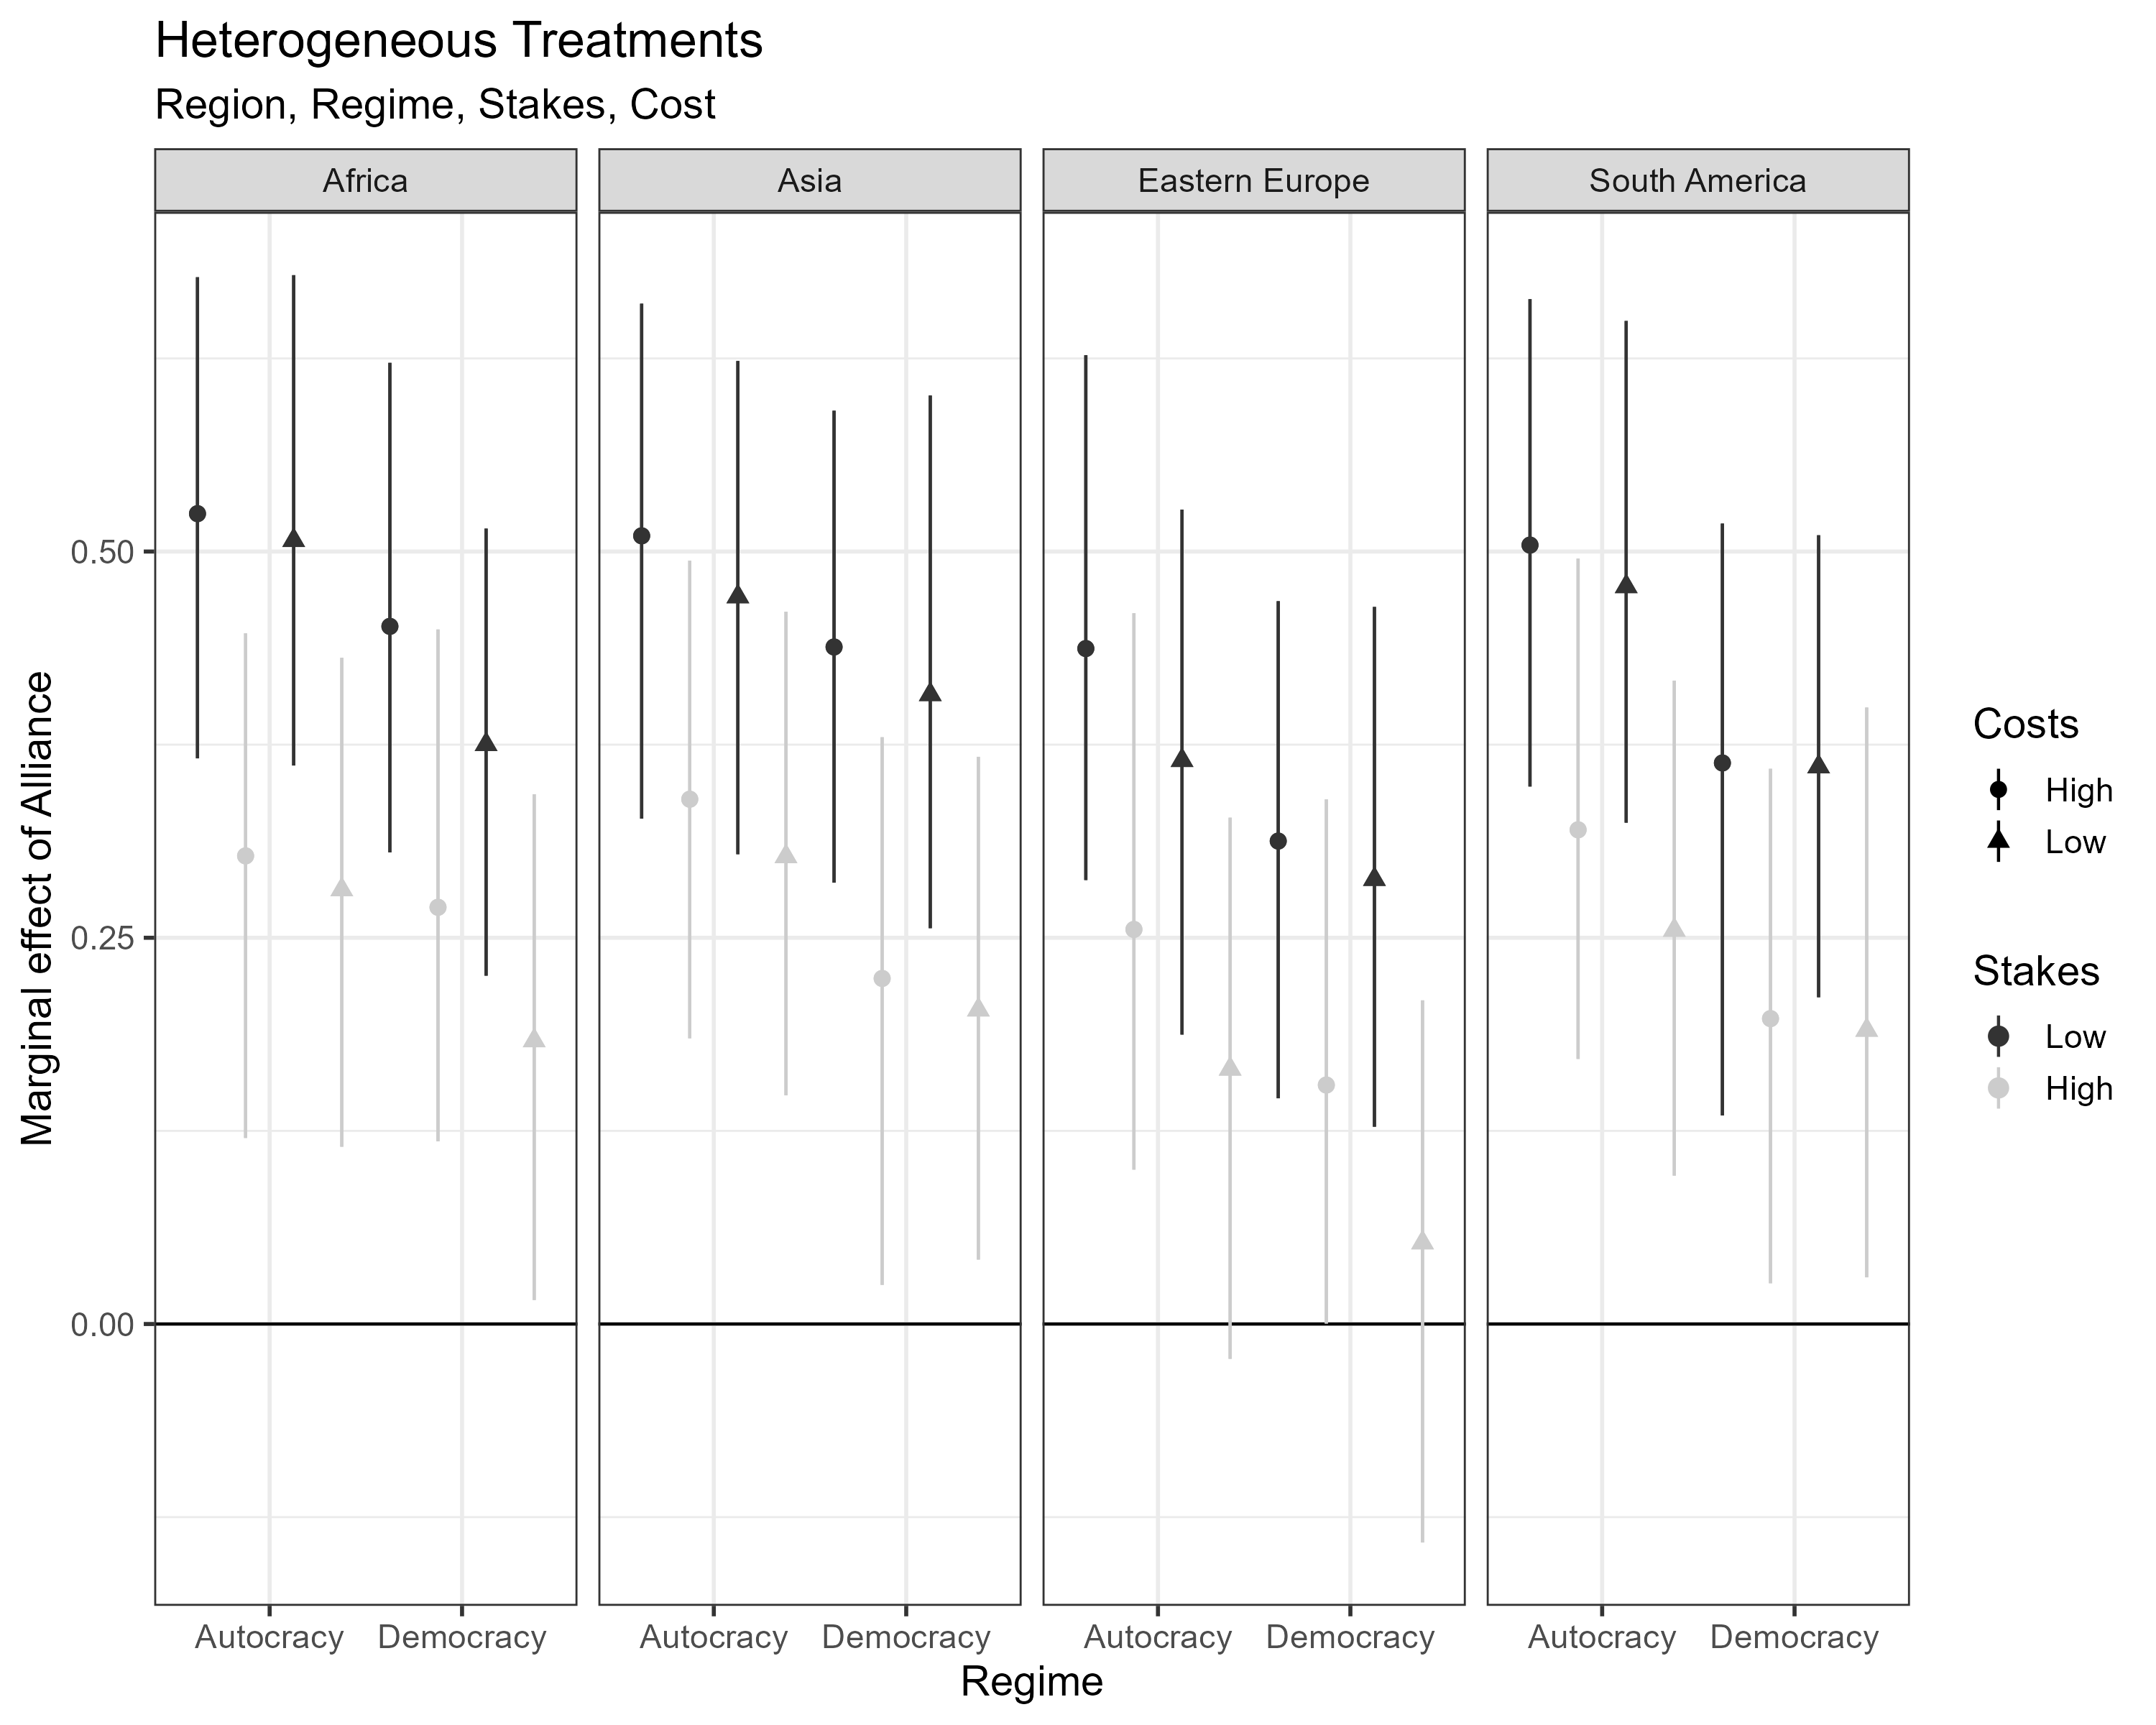
\includegraphics[width=0.95\textwidth]{../figures/tw-het-treat.png}
	\caption{Estimated impact of military alliances on public support for war across hypothetical region, costs, stakes and partner regime. Colors distinguish stakes, point shapes mark different costs, and estimates are grouped by regime type. Point estimates give the posterior median and error bars summarize the 95\% credible interval.}
	\label{fig:tw-het-treat}
\end{figure}


The impact of alliances also varies with individual respondent characteristics, as I show in \autoref{fig:tw-treat-het}. 
This uses race, gender, hawkishness and internationalism to create groups and predict the impact of alliances on support for using force. 
I selected these variables because foreign policy dispositions like militant assertiveness shape general willingness to intervene \citep{Kertzeretal2014} as does gender \citep{Barnhartetal2020} and race. 


\begin{figure}[htpb]
	\centering
		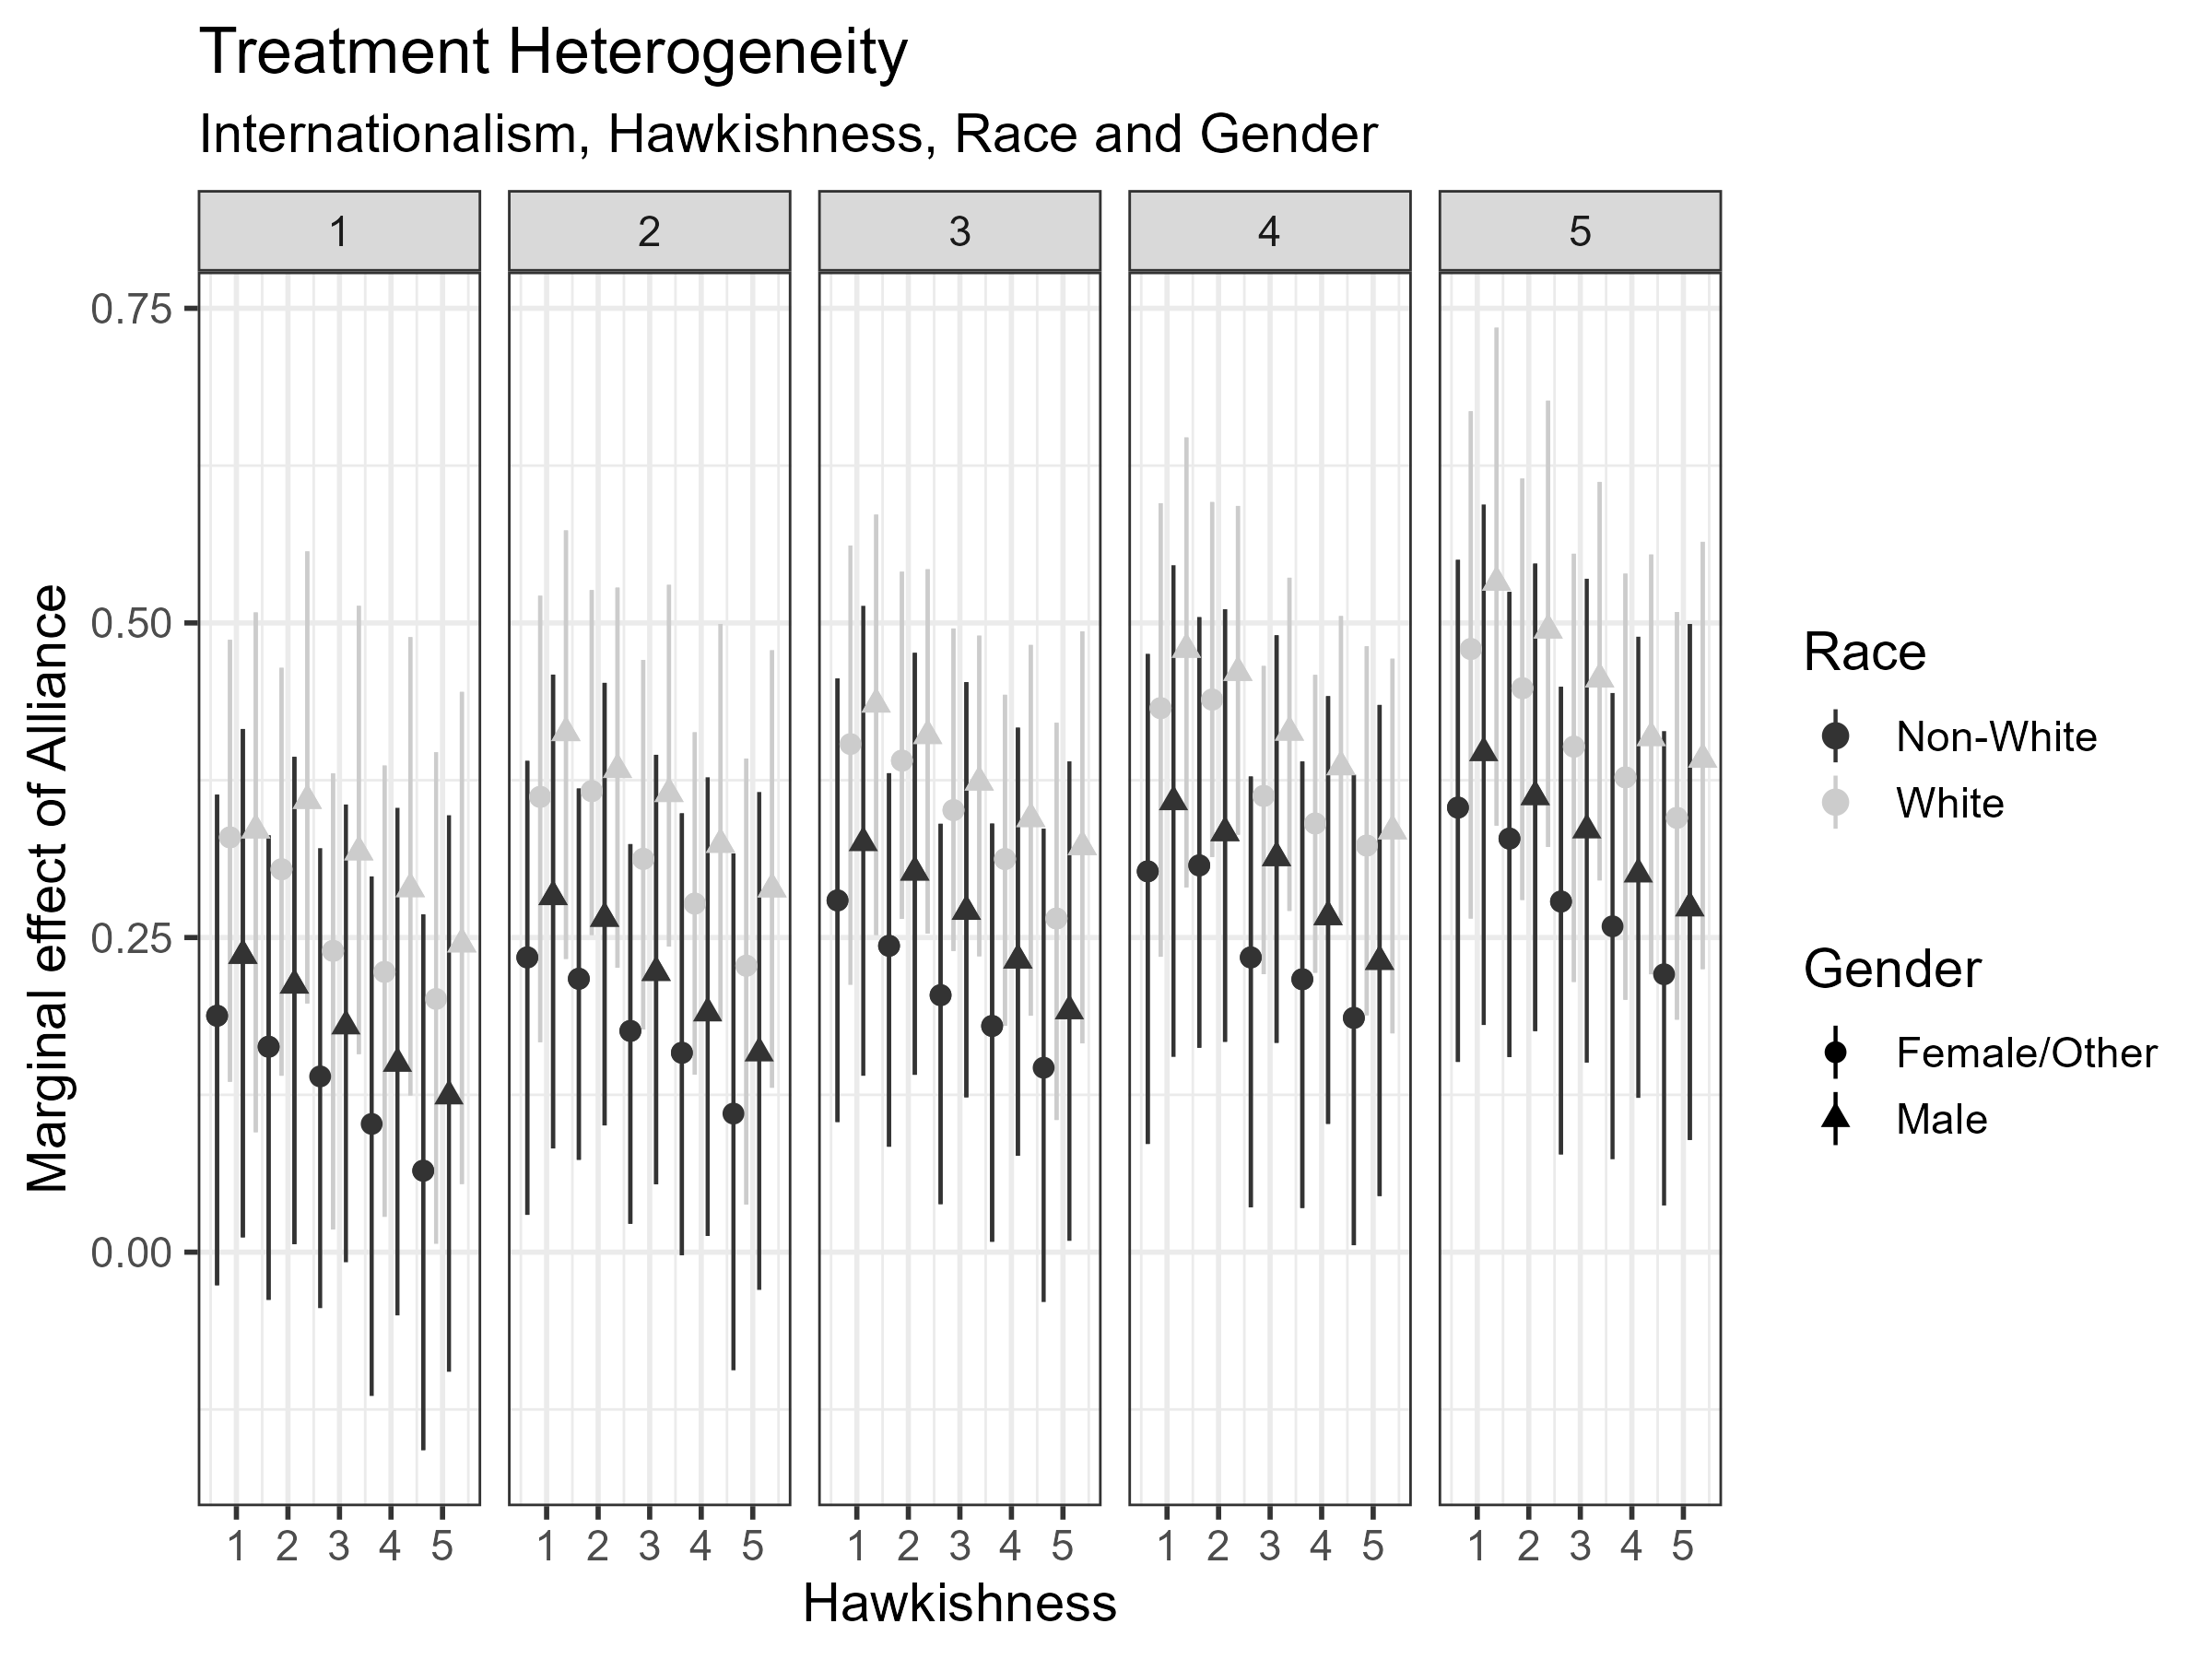
\includegraphics[width=0.95\textwidth]{../figures/tw-treat-het.png}
	\caption{Estimates of how the impact of military alliances on support for using force varies across different demographic groups. Points mark the posterior median and }
	\label{fig:tw-treat-het}
\end{figure}


The treatment heterogeneity estimates indicate that alliances exert the most influence on support for foreign interventions among white men, especially those with low hawkishness and high internationalism, who can be labeled as ``cooperative internationalists.'' 
Among white men with minimal hawkishness and maximum internationalism, alliances increase support for using force by 50\%, which is roughly double the typical effect. 
By contrast, alliances have little impact on support for war among non-white females who are skeptical of international engagement.
Militant assertiveness reduces the impact of alliances, perhaps because high militant assertiveness makes  
This implies that alliances help convince individuals who back international engagement but are less inclined to use force. 
As a result, internationalism is more important than hawkishness for understanding who is willing to fight for U.S. allies. 


These results show some of the strengths and weaknesses of the hierarchical approach to estimating heterogeneous effects. 
A relatively simple model based on demographic groups provides new insights about who responds to alliances. 
At the same time, because some demographic groups are relatively small, the within-group effect estimates can have substantial uncertainty. 
That uncertainty makes comparing groups and inferring precise effects more challenging. 
Smaller groups would have less uncertainty but perhaps average out interesting variation in the impact of alliances. 


\section{Conclusion}

This note introduced a simple and interpretable hierarchical technique for estimating heterogeneous effects. 
The approach above can apply to a wide range of outcomes, data structures, and theories. 
Explicitly modeling how different groups respond to an independent variable can help test arguments and identify who responds best to a given intervention. 


Hierarchical modeling provides an intermediate approach between simple interactions or subgroup analyses and complex machine-learning algorithms. 
As a result, this approach is a complement for existing tools, not a substitute. 
Researchers can should use this tool to check or inform other techniques.
With this and other tools, scholars and policymakers can better understand heterogeneous effects.


\singlespace
 
\bibliography{../../MasterBibliography} 


\end{document}
